\subsection{Overhead Analysis}
\label{exp:overhead}

\begin{figure}
	\centering
	\begin{minipage}{1.6in}
		% \centering
		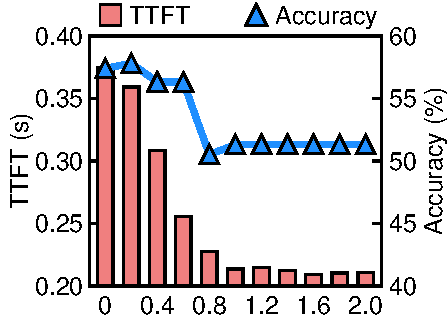
\includegraphics[width=1.6in,height=1in]{sensitivity.pdf}
		\caption{
			Results of various alpha values.
		}
		\label{fig:sensitivity_alpha}
	\end{minipage}
	\hspace{0.04in}
	\begin{minipage}{1.6in}
		\centering
		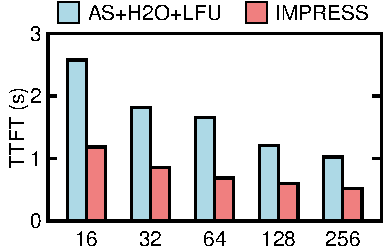
\includegraphics[width=1.6in, height=1in]{indiv_c_rte.pdf}
		\caption{
			Results of various chunk sizes.
		}
		\label{fig:sens_ck}
	\end{minipage} 
	\vspace{-0.15in}
\end{figure}

\noindent \textbf{Time overhead.} 
% The \techa{} technique in \pname{} loads the keys from the probe heads and calculates the important token index set. Although this process introduces some additional I/O and computation time, it accounts for 17\% on average in our system. 
% %This is because there are only three probe heads, so the required loading and computation are minimal.
% Additionally, the \techba{} technique sorts tokens by importance and repacks them to disk. The total execution time in our experiments is under one minute. Note that this process is asynchronous and does not affect TTFT, as it is not part of the critical path.
The \techa{} technique in \pname{} loads keys from the probe heads to determine the important token index set. While this adds some I/O and computation overhead, it averages only 6\% of our system's overhead due to the limited number of probe heads, resulting in minimal loading and computation.
Furthermore, \techba{} asynchronously sorts tokens by importance and repacks them onto disk, with a total experimental execution time of less than one minute. This process is non-intrusive to TTFT as it operates outside the critical path.

\noindent \textbf{Space overhead.} 
%\techba{} requires adding a mapping list to the metadata of each chunk to store the mapping between token positions before and after reordering. Furthermore, \techbb{} adds an extra score to each chunk. When the chunk size is 64, the total size of the mapping list and score accounts for less than 0.5\% of the chunk’s memory footprint.
%, which is acceptable. 
\fvc{
\techba{} adds a mapping list to each chunk's metadata for token position mappings post-reordering. Score-based cache management adds a score per chunk. With a 64-token chunk size, these additions account for less than 0.5\% of the chunk's memory. 
}
Additionally, to avoid loading data from other heads when loading keys from the probe heads, we redundantly store the keys from the probe heads separately. 
This accounts for 1.2\% of the total storage of all prefix KVs, which is a minimal cost considering high-capacity disks.
%Additionally, to shorten the keys from probe heads loading time, \pname{} redundantly stores them on disk, avoiding wasted disk I/O bandwidth from other heads in the same chunk. The disk space consumed by these redundant probe head stores is 1.2\% of the total prefix KV storage, which is a minimal cost considering the availability of cheap, high-capacity disks.


